\begin{figure*}
  \begin{minipage}{.5\textwidth}
    \centering
    \begin{tikzpicture}
  \node[inner sep=0pt] (two-d) at (-6,3)
  {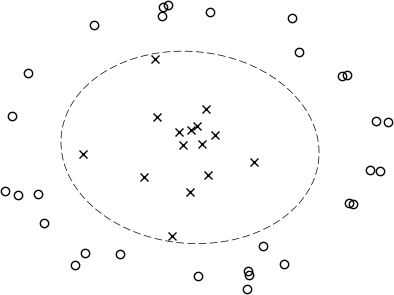
\includegraphics[width=.5\textwidth]{figure_3_3_2.png}};

  \node[inner sep=0pt] (three-d) at (-2,0)
  {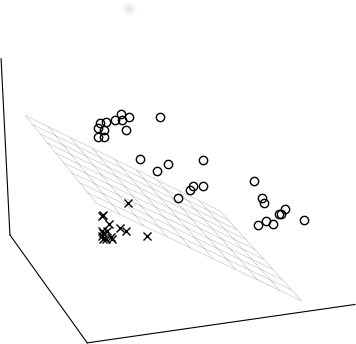
\includegraphics[width=.55\textwidth]{figure_3_2.png}};

  \draw[bend right,->]  (-7,1.6) to node [left] {$(1)$} (three-d);
  \draw[bend right,->] (-3.5,0.8) to node [right] {$(2)$} (-4.7,2.3);
    
\end{tikzpicture}

%%% Local Variables:
%%% mode: latex
%%% TeX-master: "learning_with_kernels"
%%% End:

    %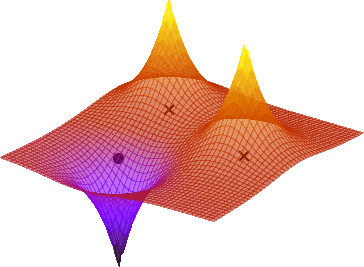
\includegraphics[width=\linewidth]{influence_map.png}
  \end{minipage}%
  \begin{minipage}{.5\textwidth}
    \centering
    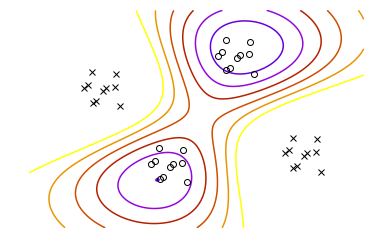
\includegraphics[width=\linewidth]{decision_boundary.png}
  \end{minipage}
  \caption{
    Le left pane illustrates how a non linear projection in a higher dimensional space makes $(1)$ it possible to learn non linear decisions boundaries in the observations space by projecting back the learned linear decision boundary $(2)$. On the right pane, the solid line represents the decision boundary and the dashed lines represents the contour levels of the decision function with learned using an RBF kernel.
  }
\end{figure*}

\section{Kernel methods}

The previous section introduced the linear SVM classifier. As we have seen, the linear SVM  allows us the find the best separating hyperplane between two linearly separable classes of observations. In this section we introduce the concept of kernels, allowing us to learn non linear decision boundaries, continuing with the \textit{Reproducing Kernel Hilbert Space} and the \textit{kernel trick}, results from functional analysis allowing us to use the newly introduced ideas of kernels with the previously presented algorithm.

\subsection{Non linearly separable data}

Very often, the decision boundary one is trying to learn is in its nature non-linear. One method that is often used to make an hyperplane learning algorithm learn a non-linear decision boundary is to first map the dataset to another space using a non linear transformation. The learned boundary is then linear in the mapped space, but because the chosen projection is not linear, the pre-image of the decision boundary is not linear.

This approach is very simple to implement and only requires light modifications the presented algorithm. Let $\phi : \mathbb{R}^n \rightarrow \mathcal{V}$ be our projection into the feature space $\mathcal{V}$. In order for the SVM algorithm to be usable, the $\mathcal{V}$ space must be a \textit{pre-Hilbert space}.

A pre-Hilbert space is a vector space equiped with a scalar product. It is simply a generalization of the usual geometrical space, the Euclidian space. This generalization allows us to work with possibly infinitly dimensional spaces, such as for instance the vector space of absolutely converging sequences $\ell_1$, the same way as we work with the more intuitive vector spaces. In this case, the optimization problem at the heart of the SVM's training algorithm is only based on the scalar product between mapped observations, thus requiring the feature space to be a pre-Hilbert space. 

We can now modify the previously introduced algorithm by replacing simply every dot product by the scalar product on the projected points in the $\mathcal{V}$ space, namely $\langle \phi(\cdot), \phi(\cdot)\rangle _{\mathcal{V}}$.

In order to better understand kernels and the kernel trick, let's analyze the example of polynomial projection of degree $d$, in which every point is projected to a vector containing every monomial of degree $d$. For instance, choosing $d = 2$ together with a $2$ dimensional input space leads to the projection $\phi : \mathbb{R}^2 \rightarrow \mathbb{R}^3$ defined as

\begin{equation*}
    \phi(x_1, x_2) \mapsto (x_1^2, x_2^2, \sqrt{2}x_1x_2)
\end{equation*}

This projection, illustrated in figure 2, makes it possible to learn a decision boundary that is not linear in the observations but it has the problem that the dimension of the image space grows at an exponential rate together with $d$, making the choice of a larger $d$ prohibitively expensive. Though, the margin maximization algorithm only uses the scalar product of the observations in the feature space, which is simply the dot product of the mapped vectors. The following equations show that the projection in the higher dimensional space is not required to the computation of the scalar product, and can be replaced by a function of the two vectors in the original space

\begin{equation*}
  \begin{aligned}
    \phi(x) \cdot \phi(\tilde{x})
    &= x_1^2\tilde{x}_1^2 + x_2^2\tilde{x}_2^2 + \sqrt{2}x_1x_2\sqrt{2}\tilde{x}_1\tilde{x}_2\\
    &= x_1^2\tilde{x}_1^2 + x_2^2\tilde{x}_2^2 + 2x_1x_2\tilde{x}_1\tilde{x}_2\\
    &= \left(x \cdot \tilde{x}\right)^2 \\
    &=: k(x, \tilde{x})
  \end{aligned}
\end{equation*}

We call $k(\cdot, \cdot) : \mathbb{R}^2 \times \mathbb{R}^2 \rightarrow \mathbb{R}$ the kernel representation of the scalar product in the space $\phi(\mathbb{R}^2)$. One can show that such a function exists for any polynomial degree $d$, making the computation of the scalar product in the $d$-th monomial space as trivial as computing the scalar product in the original space.

\subsection{Kernel trick}

We have seen in the previous example, that it is sometimes possible to find a function $k :\mathbb{R}^n \times \mathbb{R}^n \rightarrow \mathbb{R}$ with $k(x, x') = \langle \phi(x), \phi(x')\rangle _{\mathcal{V}}$ for some projection $\phi : \mathbb{R}^n \rightarrow \mathcal{V}$. With these special functions, it is possible by only lightly modifying our original algorithm to run the learning algorithm in another pre-Hilbert space without the computational cost of projecting our data in this other space. This is called the kernel trick.


We will now change our point of view and stop looking for a smart way to avoid projecting in the feature space, but instead try to define the set of functions $k$, called \textit{kernel functions}, for which it is possible to construct a pre-Hilbert space $\mathcal{V}$ and a projection $\phi$ such that $k(x, x') = \langle\phi(x), \phi(x')\rangle_{\mathcal{V}}$. This, as we will show in the next section, will make it possible to express a large variety of decision boundaries through the choice of the function.

Let $k :\mathbb{R}^n \times \mathbb{R}^n \rightarrow \mathbb{R}$, $k$ is said to be a \textit{kernel function} if the following properties hold

\begin{itemize}
\item \textit{Symmetry}
  \begin{equation*}
    \forall x_1, x_2 \in \mathbb{R}^n.\ 
    k\left(x_1, x_2\right) = k\left(x_2, x_1\right)
  \end{equation*}

\item \textit{Positive definiteness}
  \begin{equation*}
    \sum_{i,j=1}^mc_ic_jk\left(x_i, x_j\right) \geq 0
  \end{equation*}

  For any $x_1, ..., x_m \in \mathbb{R}^n$ and $c_1, ..., c_m \in \mathbb{R}$  
\end{itemize}

We now show by construction, that these properties are sufficient to the proof of the existence of the desired pre-Hilbert space. The literature contains several examples of vector spaces and projections with the desired property, but we will here prove the existence of such a space by construction.

Let $k : \mathbb{R}^n \times \mathbb{R}^n \rightarrow \mathbb{R}$ be a kernel, and $\mathbb{R}^{\mathbb{R}^n}$ be the set of functions from $\mathbb{R}^n$ to $\mathbb{R}$. We define the reproducing kernel map as follow

\begin{equation}
  \begin{aligned}
    \phi :\ &\mathbb{R}^n \rightarrow \mathbb{R}^{\mathbb{R}^n}\\
    &\mathbf{x} \mapsto k(\cdot, \mathbf{x})
  \end{aligned}
\end{equation}

Using this projection, the span of the mapped training observations constructs the following sub-vector space of functions $\mathcal{V} \subset \mathbb{R}^{\mathbb{R}^n}$

\begin{equation*}
  \begin{aligned}
    \mathcal{V}\ &:= \text{span}\left(\left\{\phi(\mathbf{x}_1), ..., \phi(\mathbf{x}_m)\right\}\right)\\    
    &= \left\{ \sum_{i=1}^m\lambda_ik(\cdot, \mathbf{x}_i)\ |\ \lambda_1, ..., \lambda_m \in \mathbb{R} \right\}
  \end{aligned}
\end{equation*}

The vector space we have constructed is a subset of the infinite dimensional vector space of functions from $\mathbb{R}^n$ to $\mathbb{R}$, but because it was constructed as the span of finitly many elements, we know that the dimension of the spanned space is at most $m$. We can now define a scalar product on $\mathcal{V}$ by first defining it on its spanning elements $\langle k(\cdot, \mathbf{x}_i), k(\cdot, \mathbf{x}_j)\rangle_{\mathcal{V}} = k(\mathbf{x}_i, \mathbf{x}_j)$. The definition can be extended on the rest of the vector space, defining the scalar product between two arbitrary functions $f = \sum_{i=1}^m\alpha_ik(\cdot, \mathbf{x}_i)$ and $g = \sum_{i=1}^m\beta_ik(\cdot, \mathbf{x}_i)$ elements of $\mathcal{V}$ as

\begin{equation}
  \begin{aligned}
    \langle f, g\rangle_{\mathcal{V}}
    &= \langle \sum_{i=1}^n\alpha_ik(\cdot, \mathbf{x}_i), \sum_{j=1}^n\beta_jk(\cdot, \mathbf{x}_j)\rangle_{\mathcal{V}} \\
    &= \sum_{i,j=1}^n\alpha_i\beta_j \langle k\left(\cdot, \mathbf{x}_i\right), k\left(\cdot, \mathbf{x}_j\right)\rangle_{\mathcal{V}} \\
    &= \sum_{i,j=1}^n\alpha_i\beta_j k\left(\mathbf{x}_i, \mathbf{x}_j\right)
    \end{aligned}
\end{equation}

The properties required for $\langle\cdot, \cdot\rangle_{\mathcal{V}}$ to be a scalar product directly follow from its definition. Bilinearity is a direct consequence of the extension of the definition to the whole span of the basis functions. As for symmetry and positive definiteness, these were set as conditions for $k$ to be a kernel function. Thus, we have constructed a pre-Hilbert space for which $k$ is equal to the scalar product of projected points

\begin{equation*}
  \begin{aligned}
    \langle \phi(\mathbf{x}_i), \phi(\mathbf{x}_j)\rangle =\ &\langle k\left(\cdot, \mathbf{x}_i\right), k\left(\cdot, \mathbf{x}_j\right)\rangle \\
    =\ &k(\mathbf{x}_i, \mathbf{x}_j)
  \end{aligned}
\end{equation*}

Now that we have presented the kernel trick as well as the existence of a corresponding pre-Hilbert space for every kernel function, the next section will focus on finding and creating useful kernels, as well as presenting some classical kernels.

\subsection {Some useful kernels}

We have defined in the last section what kernels are and how we can modify our algorithm to learn non-linear boundaries in our data. What we have omitted so far is how is one supposed to choose develop or choose a kernel when facing a practical problem.

One first way to choose a kernel is by using existing knowledge about the shape the decision boundary should have. Let's recall the equation of the decision boundary defined by the learned parameters using the kernel $k$

\begin{equation*}
  \mathscr{H} = \left\{\mathbf{x} \in \mathbb{R}^n\ |\ \sum_{\mathbf{x}_i \text{ is SV}}\alpha_iy_ik\left(\mathbf{x}, \mathbf{x}_i\right) + b = 0\right\}
\end{equation*}

For illustration, if we choose the kernel to be a polynomial kernel of degree $2$, meaning $k\left(\mathbf{x}, \mathbf{\tilde{x}}\right) = \left(\mathbf{x} \cdot \mathbf{\tilde{x}} + 1\right)^2$, we can refine the definition of the decision boundary as the set of every $\mathbf{x} \in \mathbb{R}^2$ for which following holds

\begin{equation*}
  \begin{aligned}
    0 &=\ \left(w \cdot \mathbf{x} + 1\right)^2 + b\\
      &=\ \left(w_1x_1 + w_2x_2 + 1\right)^2 + b\\
      &=\ (w_1x_1)^2 + (w_2x_2)^2 + 2w_1x_1w_2x_2 + w_1x_1 + w_2x_2 + 1 + b\\
      &=\ \mathbf{x}^T\begin{bmatrix}w_1^2 & w_1w_2\\ w_1w_2 & w_2^2\end{bmatrix}\mathbf{x} + w \cdot \mathbf{x} + 1 
  \end{aligned}
\end{equation*}

The decision boundary formed by this equation is called a quadric, the generalization of a conic section, which takes a shape from a known set of different kind of solutions. Thus, if one knows a quadric decision boundary is needed, then using a polynomial kernel of degree $2$ will learn the proper parameters of the quadric.

We have seen how previous knowledge on the shape of the decision boundary can lead to the choice of a particular kernel. Unfortunately, it is often the case that the best kind of decision boundary can't be determined. Thankfully, there is still a way to use domain knowledge about the problem to choose a kernel that will best help training a performant classifier.


In order to incorporate this other kind of domain knowledge, we have to look at kernels, not as the computations of a scalar product in some feature space, but as a similarity measurement. Taking this point of view, the kernel trick becomes a way to find the proper Hilbert space in which one's definition of similarity defines a scalar proper product, letting us use the Support Vector Machine machinery as a way to train a classifier based on our definition of similarity.

What do we mean by similarity? Let's first write down a more geometrical  definition of the euclidean scalar product in $\mathbb{R}^n$, the inner product 

\begin{equation*}
  \mathbf{x} \cdot \mathbf{\tilde{x}} = \|\mathbf{x}\|\|\mathbf{\tilde{x}}\|\text{cos}\left(angle\left(\mathbf{x}, \mathbf{\tilde{x}}\right)
  \right)
\end{equation*}

This equivalent definition of the euclidean scalar product makes it more visible what the underlying notion of similarity of the euclidean scalar product is measured by the angle between the two vectors, scaled by their length. A similar kernel often used is the cosine similarity kernel, defined as

\begin{equation*}
  k(\mathbf{x}, \mathbf{\tilde{x}}) = \frac{\mathbf{x} \cdot \mathbf{\tilde{x}}}{\|\mathbf{x}\|\|\mathbf{\tilde{x}}\|} = \text{cos}\left(angle\left(\mathbf{x}, \mathbf{\tilde{x}}\right)\right)
\end{equation*}

This notion of similarity will thus compare observations by first normalizing them to then compare the directions of the vectors. This similarity measure is often used in the context of text classification, where each entry of the vector corresponds to the number of occurences of a word in a text. The normalization will transform count of occurences in frequencies, thus having a similarity based on the relative importance of each word, independently of the length of the text.

Cosine similarity is an interesting similarity, but one natural way to reason about similarity of points is their distance from one another. The next kernel we introduce incorporates the notions of distance as a similarity measurement, is called the Radial Basis Function kernel and is defined as followed for some hyperparameter $\sigma \in \mathbb{R}$

\begin{equation*}
  k(\mathbf{x}, \mathbf{\tilde{x}}) = \text{exp}\left(-\frac{\|\mathbf{x} - \mathbf{\tilde{x}}\|^2}{\sigma^2}\right)
\end{equation*}

This kernel contains the idea that similarity between two observations should decay exponentially with the distance between the two vectors. This kernel isn't only a good model of our notion of similarity, but it also has interesting properties when used with the Support Vector Machines training algorithm.

Let's first recall what was the decision function that was learned by the algorithm

\begin{equation*}
  f\left(x\right) = sgn\left(\sum_{\mathbf{x}_i \text{ is SV}}\alpha_iy_ik\left(\mathbf{x}, \mathbf{x}_i\right) + b\right)
\end{equation*}

We evaluate the sign of a linear combination of the similarity of the current observation to the support vectors. One can see understand each support vector as a point of influence in the direction of the class it belongs to, with it's influence intensity exponentially decaying with the distance. The observation will then be classified by taking a weighted sum of the influence of each support vector and verifying if it is over or under some threshold $b$.

We have shown with three examples how previous knowledge can help train high quality classifiers. Because we had to omit many interesting concepts of choice of kernel, the reader is invited to consult further resources to learn about more mechanical ways to construct kernels \cite{Scholkopf:2001:LKS:559923} but also about invariane incorporation \cite{Decoste2002} or advanced approach in kernel design for solving modern complex problems \cite{lauer:hal}.

%%% Local Variables:
%%% mode: latex
%%% TeX-master: "learning_with_kernels"
%%% End:
